\section{Auswertung} % (fold)
\label{sec:swrtng}


\subsection{Bestimmung der Winkelrichtgröße $D$}
\begin{table}
	\centering
	\def\arraystretch{1.3} 
	\begin{tabular}{ccc}
	\toprule
	\multicolumn{2}{c}{Winkel} & {Kraft} \\
	{$\phi$} & {$\phi/\:\text{rad}$} & {$F/\:\si{\newton}$} \\
	\midrule
 45$\text{°}$ & $\frac{\pi}{4}$   & 0.22 \\ 
 90$\text{°}$ & $\frac{\pi}{2}$   & 0.40 \\
120$\text{°}$ & $\frac{2\pi}{3}$  & 0.52 \\
135$\text{°}$ & $\frac{3\pi}{4}$  & 0.60 \\
180$\text{°}$ & $\pi$             & 0.78 \\
225$\text{°}$ & $\frac{5\pi}{4}$  & 0.92 \\
240$\text{°}$ & $\frac{4\pi}{3}$  & 0.90 \\
270$\text{°}$ & $\frac{3\pi}{2}$  & 1.08 \\
315$\text{°}$ & $\frac{7\pi}{4}$  & 1.26 \\
360$\text{°}$ & $2\pi$            & 1.42 \\
	\bottomrule
	\end{tabular}
	\label{tab:M1 I_D}
	\caption{Messung zur Bestimmung des Eigenträgheitsmomentes der Drillachse.}
\end{table}

\noindent Mit den Messwerten und $r=0.09965\si{\meter}$ lässt sich die Winkelrichtgröße $D$ mit der Gleichung \eqref{eq:Winkelricht} bestimmen. Die Unsicherheit ist die Standardabweichung des Mittelwertes $\sigma_D$ mit
\begin{subequations}
	\begin{equation}
		\sigma_x = \sqrt{\sigma_x^2} := \sqrt{\frac{1}{n^2-n} \sum_{i=1}^n{(x_i-\bar{x})^2}}
	\end{equation}
	\begin{equation}
		\bar{x} = \frac{1}{n} \sum_{i=1}^n{x_i}.
	\end{equation}
\end{subequations}
für $x=D$.
Es ergibt sich 
\begin{equation}
	\label{wert:Winkelricht}
	D=(0.0757\pm0.0019)\si{\newton\meter}
\end{equation}
\subsection{Bestimmung des Eigenträgheitsmomentes $I_D$}
\begin{table}[hp]
	\centering
	\sisetup{table-format=2.3}
	\begin{tabular}{S[table-format=2.4] S[table-format=2.2] S[table-format=1.3] S[table-format=2.2] S[table-format=1.3] S[table-format=3.2] S[table-format=3.2]}
	\toprule
	{Abstand}&\multicolumn{4}{c}{Schwingungsdauer} & \multicolumn{2}{c}{Masse} \\
	{$a/\:\si{\centi\meter}$} & {$2T_{1}/\:\si{\second}$} & {$T_{1}/\:\si{\second}$} & {$2T_{2}/\:\si{\second}$} & {$T_{2}/\:\si{\second}$} & {$m_{1}/\:\si{\gram}$} & {$m_{2}/\:\si{\gram}$}\\
	\midrule
 6.4925 &  5.90 & 2.950 &  5.90 & 2.950 & 221.74 & 221.73 \\
 8.4925 &  6.55 & 3.275 &  6.46 & 3.230 & 221.74 & 221.73 \\
10.9925 &  7.29 & 3.645 &  7.21 & 3.605 & 221.75 & 221.73 \\
13.7925 &  8.66 & 4.330 &  8.63 & 4.315 & 221.76 & 221.75 \\
16.6925 & 10.07 & 5.035 & 10.10 & 5.050 & 221.75 & 221.74 \\
19.0925 & 11.13 & 5.565 & 11.15 & 5.575 & 221.75 & 221.74 \\
20.4925 & 11.92 & 5.960 & 11.76 & 5.880 & 221.75 & 221.73 \\
22.4925 & 13.03 & 6.515 & 13.00 & 6.500 & 221.76 & 221.74 \\
24.5925 & 14.10 & 7.050 & 13.96 & 6.980 & 221.75 & 221.75 \\
29.5925 & 16.67 & 8.335 & 16.73 & 8.365 & 221.76 & 221.74 \\
	\bottomrule
	\end{tabular}
	\caption{Messung zur Bestimmung des Eigenträgheitsmomentes der Drillachse}\label{tab:M2 I_D}
\end{table}
Zur Bestimmung des Eigenträgheitsmomentes $I_D$ wird die verwendete Stange als nahezu masselos angenommen, 
wodurch ihr Anteil am Trägheitsmoment vernachlässigbar ist. 
Das gemessene Trägheitsmoment setzt sich aufgrund der Linearität des Trägheitsmomentes aus den Trägheitsmomenten der Massestücke $m_1$ und $m_2$ als Punktmassen, sowie dem Eigenträgheitsmoment $I_D$ zusammen,
\begin{equation}
	I= I_D+I_{m_1}+I_{m_2}.
\end{equation}
Nach Einsetzen in Gleichung \eqref{eq:Winkelricht} wird der lineare Zusammenhang von $T^2$ und $a^2$ ersichtlich.
Es gilt
\begin{align*}
	 D &= 4\mathup{\pi^{2}}\cdot\frac{I}{T^2}\\
	   &= 4\mathup{\pi^{2}}\cdot\frac{I_D+I_{m_1}+I_{m_2}}{T^2}\\
	   &= 4\mathup{\pi^{2}}\cdot\frac{I_D+a^{2}(m_1+m_2)}{T^2}\\
	T^2&= 4\mathup{\pi^{2}}\frac{I_D}{D}+4\mathup{\pi^{2}}\frac{a^{2}(m_1+m_2)}{D}\\
\end{align*}
\begin{equation}
	\label{eq:Reg_ident}
	T^2= \underbrace{4\mathup{\pi^{2}}\frac{(m_1+m_2)}{D}}_{m_{\text{Reg}}}\cdot a^{2}+\underbrace{4\mathup{\pi^{2}}\frac{I_D}{D}}_{b_{\text{Reg}}}
\end{equation}
Zur Bestimmung des Eigenträgheitsmoments $I_D$ werden die gemittelten Schwingperioden-Quadrate ${T}^2$ gegen das Abstandsquadrat $a^2$ aufgetragen. Aus der Regression mittels der Formeln
\begin{subequations}
	\begin{equation}
		\Delta = N \sum{x^2} - {(\sum{x})}^2
	\end{equation}
	\begin{equation}
		m_{\text{Reg}} = \frac{N\sum{x\cdot y} - \sum{x} \cdot \sum{y}}{\Delta}
	\end{equation}
    \begin{equation}
		b_{\text{Reg}} = \frac{\sum{x^2} \cdot \sum{y} - \sum{x} \cdot \sum{x \cdot y}}{\Delta}
	\end{equation}
	\begin{equation}
		\sigma_{y} = \sqrt{\frac{\sum{(y - m_{\text{Reg}} \cdot x - b_{\text{Reg}})^2}}{N - 2}}
	\end{equation}
	\begin{equation}
		\sigma_{m} = \sigma_{y} \sqrt{\frac{N}{\Delta}}
	\end{equation}
	\begin{equation}
		\sigma_{b} = \sigma_{y} \sqrt{\frac{\sum{x^2}}{\Delta}}
	\end{equation}
\end{subequations}
für $x=a^2$, $y=T^2$ und der Identität aus Gleichung \eqref{eq:Reg_ident}, wird das Eigenträgheitsmoment $I_D$ berechnet
\begin{equation*}
	I_D= \frac{D}{4\mathup{\pi^2}}b_{\text{Reg}}\\
\end{equation*}
\begin{equation}
	\label{wert:eigentragheit}
	= (9.26\pm0.23)10^{-3} \si{\kilo\gram\meter\squared}
\end{equation}
Da dieses Trägheitsmoment größer ist als die Ergebnisse der folgenden Messungen, wird von dem Abzug des Eigenträgheitsmomentes abgesehen (vgl. Kapitel \ref{Systembestimmend}).
\begin{figure}[hp]
	\centering
	\label{fig:Regress}
	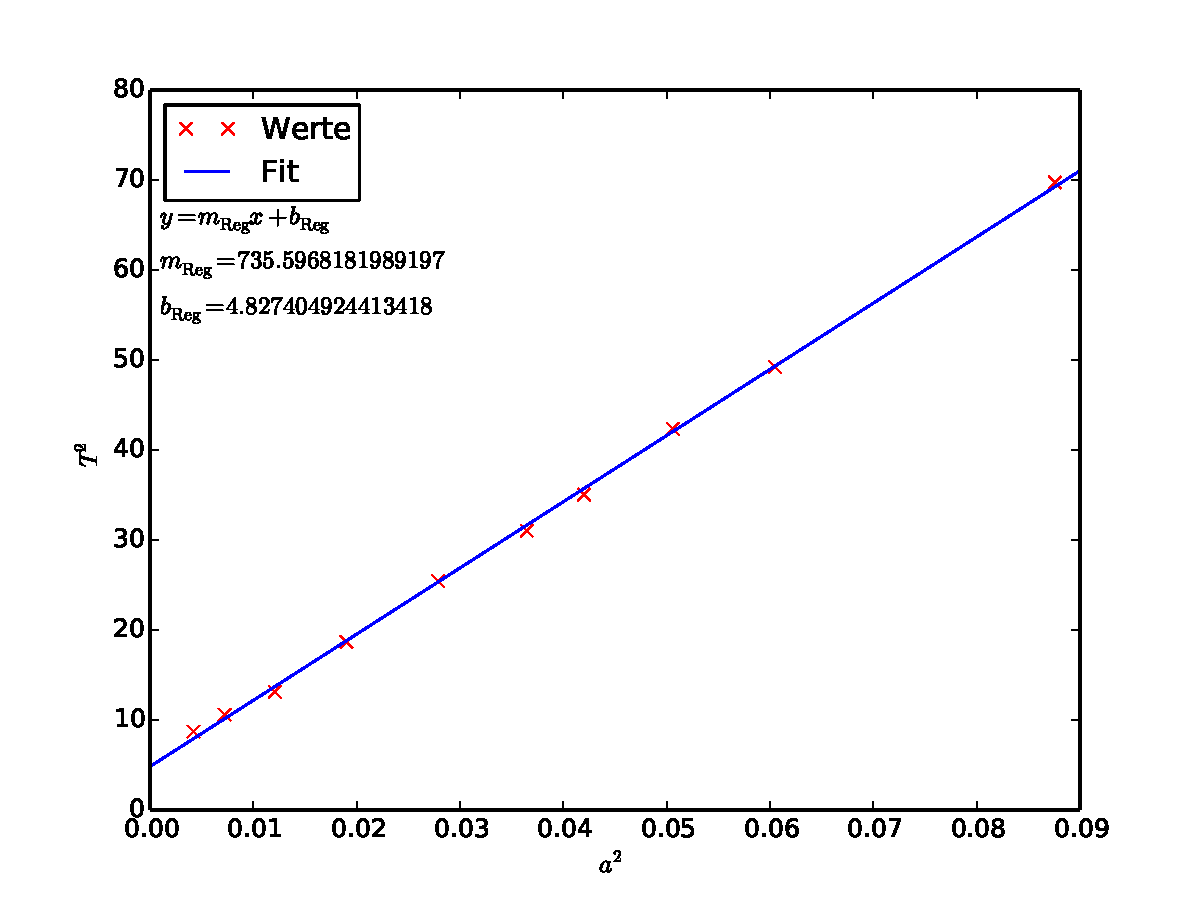
\includegraphics[width=\textwidth]{Bilder/Messung2.pdf}
	\caption{Regression von $T^2$ gegen $a^2$}
\end{figure}
\newpage
\subsection{Trägheitsmoment $I_\text{Z}$ eines Zylinders}
\label{sub:traegheitsmoment_eines_zylinders}
\begin{table}
	\centering
	\sisetup{table-format=2.3}
	\begin{tabular}{S[table-format=1.2] S[table-format=1.3] S[table-format=2.3] S[table-format=1.3] S[table-format=3.2]}
	\toprule
	\multicolumn{2}{c}{Schwingungsdauer} & \multicolumn{2}{c}{Abmessungen}&{Masse}\\

{$5T/\:\si{\second}$} & {$T/\:\si{\second}$} & {$\text{Höhe}\:H/\:\si{\centi\meter}$} & {$\text{Durchmesser}\:D/\:\si{\centi\meter}$} & {$M/\:\si{\gram}$}\\
	\midrule
4.41 &  0.882 &	10.120	& 9.848	& 368.57 \\
4.35 &	0.870 & 10.150	& 9.850	& 368.57 \\
4.44 &	0.888 & 10.120	& 9.844	& 368.57 \\
4.44 &	0.888 & 10.102	& 9.840	& 368.57 \\
4.36 &	0.872 & 10.112	& 9.844	& 368.57 \\
4.41 &  0.882 &	10.112	& 9.850	& 368.58 \\
4.32 &	0.864 & 10.058	& 9.850	& 368.59 \\
4.40 &	0.880 & 10.070	& 9.844	& 368.57 \\
4.33 &	0.886 & 10.068	& 9.844	& 368.58 \\
4.39 &  0.878 &	10.072	& 9.850	& 368.57 \\
	\bottomrule
	\end{tabular}
	\caption{Messung zur Bestimmung des Eigenträgheitsmomentes eines Zylinders}
	\label{tab:M3 I_Z}
\end{table}
\noindent Mit bekannter Winkelrichtgröße $D$ wird die Gleichung \eqref{eq:Winkelricht} benutzt, um das Trägheitsmoment aus der Schwingungsdauer $T$ zu berechnen. Der Fehler des Trägheitsmomentes wird mithilfe der Gausschen Fehlerfortpflanzung mit
\begin{equation}
	\label{eq:Gauss}
	\sigma=\sqrt{\sum_i^N{\left( \frac{\partial{f}}{\partial{x_i}}\right)^2\m \Delta x_i^2}}
\end{equation}bestimmt.
Es ergibt sich
\begin{equation}
	\label{wert:Zylinder}
	I_\text{Z} = (1.48\pm0.04)10^{-3} \si{\kilo\gram\meter\squared}
\end{equation}
Das sichtbare Material der Zylinders ist Styropor-ähnlich. 
Da die gemessene Masse des Zylinders, $m_\text{Z} = (368.5740\pm0.0022) \si{\gram}$, stark von der theoretischen Masse eines Styropor-Zylinders gleicher Maße, $m_\text{Theorie} = \mathup{\rho_{\text{Styropor}}}V=(807.4\pm0.8) \si{\gram}$, abweicht, 
wird die Vermutung angestellt, dass der Körper ein Hohlzylinder ist oder dass der Körper nicht vollständig aus Styropor besteht.
\begin{figure}[b]
	\label{fig:tonne}
	\centering
	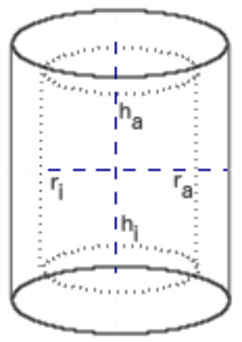
\includegraphics[scale=0.5]{Bilder/Tonne.pdf}
	\caption{Bezeichnungen des Hohlzylinders}
\end{figure}
Zur Bestimmung der Geometrie des vermuteten Styropor-Hohlzylinders wird die Formel für Hohlzylinder-Volumen  mit der Dichte $\mathup{\rho_{\text{Styropor}}}$ multipliziert und mit der gemessenen Masse gleichgesetzt. 
Dabei gilt die Annahme, dass die Stärke des Hohlzylinders für Mantel, Deckel und Boden gleich sind, $r_a-r_i=h_a-h_i$. 
Die so von zwei Unbekannten $r_i$ und $h_i$ auf eine Unbekannte $r_i$ reduzierte Gleichung
\begin{equation}
	m_\text{Z}=\rho(-2\pi*(r_i)^3+(r_i)^2*(2\pi r_a-\pi h_a)+(\pi h_a r_a^2)
\end{equation}
ergibt für den Innenradius $r_i = 0.0401012\si{\meter}\pm0.0898\%$.
Das Trägheitsmoment eines solchen Hohlzylinders setzt sich zusammen aus den Trägheitsmomenten eines Zylindermantels und zwei Kreisscheiben, die um ihren Mittelpunkt rotieren.
\begin{table}[h]
	\centering
	\sisetup{table-format=2.3}
	\begin{tabular}{ccc}
	\toprule
	&{Mantel}&{Kreisscheibe}\\
	\midrule
{Volumen / $\si{\meter\cubed}$}&$0.0002588\pm0.0000010$&$(4.613\pm0.010)10^{-5}$\\
{Masse / $\si{\kilo\gram}$}&$0.2717\pm0.0010$&$0.04844\pm0.00011$\\
{Trägheitsmoment / $\si{\kilo\gram\meter\squared}$}&$0.0005478\pm0.0000017$&$(3.8945\pm0.0028)10^{-5}$\\
	\bottomrule
	\end{tabular}
	\caption{Daten des angenommenen Hohlzylinders}
	\label{tab:M3 I_Z}
\end{table}

Es gilt
\begin{align*}
	I_{\text{HZ, Theorie}}&=I_{\text{Zylindermantel}}+2I_{\text{Kreisscheibe}}\\
	&=m_\text{Mantel} \frac{r_i^2+r_a^2}{2}+m_\text{Kreisscheibe} r_i^2
\end{align*}
und es ergibt sich
\begin{equation}
	I_{\text{HZ, Theorie}}= (6.257\pm.0017)10^{-4} \si{\kilo\gram\meter\squared}
\end{equation}
\subsection{Trägheitsmoment $I_\text{K}$ einer Kugel}
\begin{table}
	\centering
	\sisetup{table-format=2.3}
	\begin{tabular}{S[table-format=1.2] S[table-format=1.3] S[table-format=1.3] S[table-format=3.1]}
	\toprule
	\multicolumn{2}{c}{Schwingungsdauer} & {Abmessungen} & {Masse} \\
	{$5T/\:\si{\second}$} & {$T/\:\si{\second}$} & {$\text{Durchmesser}\:D/\:\si{\centi\meter}$} & {$M/\:\si{\gram}$}\\
	\midrule
8.60 & 1.720 & 13.745 &	812.7 \\
8.56 & 1.721 & 13.730 &	812.7 \\
8.61 & 1.722 & 13.720 &	812.7 \\
8.58 & 1.716 & 13.745 &	812.7 \\
8.56 & 1.721 & 13.750 &	812.7 \\
8.61 & 1.722 & 13.740 &	812.7 \\
8.55 & 1.710 & 13.750 &	812.7 \\
8.61 & 1.722 & 13.710 &	812.7 \\
8.60 & 1.720 & 13.745 &	812.7 \\
8.61 & 1.722 & 13.730 &	812.7 \\
	\bottomrule
	\end{tabular}
	\caption{Messung zur Bestimmung des Eigenträgheitsmomentes einer Kugel}
	\label{tab:M4 I_K}
\end{table}
\noindent Analog zu \ref{sub:traegheitsmoment_eines_zylinders} wird über die Schwingungsdauer $T$ das Trägheitsmoment $I_\text{K}$ der Kugel zu
\begin{equation}
	\label{wert:Kugel}
	I_K=(5.67\pm0.14)10^{-3} \si{\kilo\gram\meter\squared}
\end{equation}
bestimmt.
Für die theoretische Berechnung des Trägheitsmomentes wird die gemessene Masse der Kugel benutzt.
Mit $I_K = \frac{2}{5} m_{\text{Kugel}} r^2$ ist 
\begin{equation}
	\label{wert:Kugel}
	I_\text{K, Theorie}= (1.5335\pm0.0010)10^{-3} \si{\kilo\gram\meter\squared}
\end{equation}
\subsection{Trägheitsmoment $I_\text{Puppe}$}
\begin{table}[h]
	\centering
	\sisetup{table-format=1.2}
	\begin{tabular}{SS}
	\toprule
	{Position (2)/s}&{Position (1)/s}	\\
	\midrule
	  	0.974 	&0.768\\
	  	0.956	&0.778\\
	  	0.974	&0.772\\
	  	0.960	&0.772\\
	  	0.972	&0.774\\
	  	0.992	&0.786\\
	 	0.960	&0.768\\
	  	0.980	&0.780\\
		0.980	&0.768\\
		0.974	&0.774\\
	\bottomrule
	\end{tabular}
	\caption{Schwingungsdauer der Puppe}
	\label{tab:M6 Puppenzeit}	
\end{table}

\noindent Analog zu \ref{sub:traegheitsmoment_eines_zylinders} wird über die Schwingungsdauer $T$ das Trägheitsmoment $I_\text{Puppe}$ für beide Positionen zu
\begin{subequations}
	\begin{equation}
		\label{wert:Puppe1}
		I_\text{Puppe,1}=(1.81\pm0.04)10^{-3} \si{\kilo\gram\meter\squared}
	\end{equation}
	\begin{equation}
		\label{wert:Puppe2}
		I_\text{Puppe,2}=(1.149\pm0.028)10^{-3} \si{\kilo\gram\meter\squared}
	\end{equation}
\end{subequations}
bestimmt.
Für die theoretische Berechnung werden die Volumina der Körperteile, die Dichte der Puppe $\rho_\text{Puppe}$ 
mit $\rho_\text{Puppe}=\frac{m_\text{Puppe}}{V_\text{Puppe, Gesamt}}$ und dadurch die Massen der Körperteile bestimmt. 
Die Daten sind der Tabelle \ref{tab:M6 Puppenzeit} zu entnehmen.
Für die Einzelträgheitsmomente, deren Summe das Trägheitsmoment der Puppe ist, gelten die Formeln
\begin{align*}
	I_\text{Arm,1} &= \frac{m_\text{Arm}}{2}\Bigl(\frac{d_\text{Arm}}{2}\Bigr)^2+\underbrace{m_\text{Arm}\Bigl(\frac{d_\text{Rumpf}}{2}+\frac{d_\text{Arm}}{2}\Bigr)^2}_{\text{Satz von Steiner}}\\
	I_\text{Arm,2} &= \frac{m_\text{Arm}}{2}(\frac{d_\text{Arm}}{2})^2\\
	I_\text{Bein} &= m_\text{Bein}\Bigl(\frac{(d_\text{Bein})^2}{16}+\frac{(h_\text{Bein})^2}{12}\Bigr)+
	\underbrace{m_\text{Bein}\Bigl(\frac{h_\text{Bein}}{2}\Bigr)^2}_{\text{Satz von Steiner}}\\
	I_\text{Kopf} &= \frac{2m_\text{Kopf}}{5}\Bigl(\frac{d_\text{Kopf}}{2}\Bigr)^2\\
	I_\text{Rumpf} &= \frac{m_\text{Rumpf}}{2}\Bigl(\frac{d_\text{Rumpf}}{2}\Bigr)^2
\end{align*}
\begin{landscape}
	\centering
	\begin{table}[p]
	\centering
	\begin{tabular}{S[table-format=1.1] S[table-format=1.1] S[table-format=2.1] S[table-format=2.1] S[table-format=1.1] S[table-format=1.1] S[table-format=2.1] S[table-format=2.1] S[table-format=1.1] S[table-format=1.1] S[table-format=2.1] S[table-format=3.2]}
		\toprule
		\multicolumn{2}{c}{Armdurchmesser} & \multicolumn{2}{c}{Armlänge} & \multicolumn{2}{c}{Beindurchmesser} & \multicolumn{2}{c}{Beinlänge} & {Kopf} & \multicolumn{2}{c}{Rumpf} & {Masse}\\
		{links} &{rechts} &{links} &{rechts} &{links} &{rechts} &{links} &{rechts}\\
		{$d_{\text{A}}/\:\si{\centi\meter}$} & {$d_{\text{A}}/\: \si{\centi\meter}$} & {$l_{\text{A}}/\:\si{\centi\meter}$} & {$l_{\text{A}}/\: \si{\centi\meter}$} & {$d_{\text{B}}/\:\si{\centi\meter}$} & {$d_{\text{B}}/\: \si{\centi\meter}$} & {$l_{\text{B}}/\: \si{\centi\meter}$} & {$l_{\text{B}}/\:\si{\centi\meter}$} & {$d/\si{\centi\meter}$} & {$d/\si{\centi\meter}$} & {$l/\si{\centi\meter}$} & {$M/\si{\gram}$}\\
		\midrule
		1.7 &	1.5 &	14.1 & 	14.0 & 	1.6 & 	1.6 &	15.0 &   15.5 & 3.0 &	3.9		&  9.9	& 162.60 \\
		1.3 &	1.4 & 	14.2 & 	14.1 & 	1.7 & 	2.1 &  	14.9 &   15.4 & 3.0 &	3.6 	& 10.0	& 162.61 \\	
		1.6 &	1.6 & 	14.0 & 	14.0 & 	2.0 & 	1.8 &  	15.0 &   15.4 & 3.1 &	3.6 	&  9.9	& 162.62 \\
		1.0 &	1.2 & 	13.9 & 	14.1 & 	1.2 & 	1.6 &  	15.0 &   15.6 & 3.1 &	3.9  	&  9.9	& 162.65 \\
		1.4 &	1.1	& 	14.0 & 	13.9 & 	1.7 & 	1.1 &  	14.9 &   15.6 & 3.0 &	4.1		&  9.9	& 162.63\\
		0.9 &	1.4	& 	13.8 & 	14.1 & 	1.4 & 	1.5 &  	14.9 &   15.6 & 3.1 &	3.5		& 10.0	& 162.63 \\
		1.6 &	1.3	& 	13.9 & 	14.0 & 	1.3 & 	1.3 &  	15.0 &   15.3 & 3.0 &	3.7		&  9.8	& 162.61 \\
		1.5 &	1.1	& 	14.1 & 	14.1 & 	1.9 & 	1.0 &  	14.9 &   15.4 & 3.1 &	3.5		&  9.9	& 162.62 \\
		1.6 &	0.9	& 	13.8 & 	14.1 & 	1.5 & 	1.7 &  	15.0 &   15.6 & 3.0 &	3.6		&  9.7	& 162.61 \\
		1.7 &	1.4	& 	13.9 & 	14.2 & 	1.3 & 	1.6 &  	15.0 &   15.6 & 3.1 &	3.2		&  9.8	& 162.64 \\
		\bottomrule
	\end{tabular}
	\caption{Abmessungen und Masse der Modellpuppe}
	\label{tab:M5.1 Abmessungen Puppe}	
\end{table}
	\begin{table}[p]
	\centering
	\begin{tabular}{ccccccc}
	\toprule
	&\multicolumn{2}{c}{Arm} & \multicolumn{2}{c}{Beine}  & {Kopf} & {Rumpf}\\
	&{links} &{rechts} &{links} &{rechts} &{} & {}\\
	\midrule
	Volumen/$10^{-5}\si{\meter\cubed}$&$2.24 \pm0.28$ &$1.84 \pm0.19$&$2.86 \pm0.31 $&$2.8 \pm0.4 $&$1.486 \pm0.024$ &$9.8 \pm0.7$\\
	Masse/\si{\kilo\gram} &$0.0173 \pm0.0021$&$0.0142 \pm0.0015$&$0.0220 \pm0.0023$&$0.0220 \pm0.0027$&$0.0114 \pm0.0005$&$0.076 \pm0.004$\\
	\bottomrule
	\end{tabular}
	\caption{Abmessungen und Masse der Puppenteile}
	\label{tab:M6 Puppenteile}	
\end{table}
\end{landscape}
\begin{table}[ht]
	\centering
	\begin{tabular}{lc}
	\toprule
	\multicolumn{2}{c}{Trägheitsmoment /$10^{-5}\cdot\si{\kilo\gram\meter\squared}$}\\
	\midrule
	Linker Arm Pos.1 &$1.12\pm0.17$\\
	Rechter Arm Pos.1 &$0.86\pm0.011$\\
	Linker Arm Pos.2 &$16.10\pm1.9$\\
	Rechter Arm Pos.2 &$13.30\pm1.4$\\
	Linkes Bein&$16.5\pm1.7$\\
	Rechtes Bein&$17.6\pm2.2$\\
	Kopf&$0.106\pm0.006$\\
	Rumpf&$1.20\pm0.14$\\
	\bottomrule
	\end{tabular}
	\caption{Trägheitsmomente der Puppenteile.}
	\label{tab:M8 Tragheit}	
\end{table}

\noindent Damit ergeben sich die theoretischen Gesamtträgheitsmomente 
\begin{subequations}
	\label{wert:Puppe1T}
	\begin{align}
		I_\text{Puppe,1,Theorie}=(6.48\pm0.27)10^{-4}  \si{\kilo\gram\meter\squared},\\
		I_\text{Puppe,2,Theorie}=(3.74\pm0.24)10^{-4} \si{\kilo\gram\meter\squared}.
	\end{align}
\end{subequations}
Der Quotient $\alpha$ der theoretischen Trägheitsmomente aus \eqref{wert:Puppe1T} ist
\begin{subequations}
	\begin{align}
		\label{eq:Quo1}
		\alpha = \frac{I_\text{Puppe,1,Theorie}}{I_\text{Puppe,2,Theorie}}=1.73\pm0.08,
		\intertext{analog ist der Quotient $\beta$ der gemessenen Trägheitsmomente aus \eqref{wert:Puppe1} und  \eqref{wert:Puppe2}} 
	\label{eq:Quo2}
		\beta = \frac{I_\text{Puppe,1}}{I_\text{Puppe,2}}\approx1.58.
		\end{align}
\end{subequations}
Ausgehend von der Unsicherheit von $D$ (vgl. Gleichung \eqref{wert:Winkelricht}) und in $T$ (vgl. Gleichung \eqref{tab:M6 Puppenzeit}), ist die Unsicherheit von \beta mit $2.0\cdot10^{-15}\%$ ist vernachlässigbar.
% subsection traegheitsmoment_eines_zylinders (end)
% section auswertung (end)
